%Version 3.1 December 2024
% See section 11 of the User Manual for version history
%%%%%%%%%%%%%%%%%%%%%%%%%%%%%%%%%%%%%%%%%%%%%%%%%%%%%%%%%%%%%%%%%%%%%%
%%                                                                 %%
%% Please do not use \input{...} to include other tex files.       %%
%% Submit your LaTeX manuscript as one .tex document.              %%
%%                                                                 %%
%% All additional figures and files should be attached             %%
%% separately and not embedded in the \TeX\ document itself.       %%
%%                                                                 %%
%%%%%%%%%%%%%%%%%%%%%%%%%%%%%%%%%%%%%%%%%%%%%%%%%%%%%%%%%%%%%%%%%%%%%
%%\documentclass[referee,sn-basic]{sn-jnl}% referee option is meant for double line spacing

%%=======================================================%%
%% to print line numbers in the margin use lineno option %%
%%=======================================================%%

%%\documentclass[lineno,pdflatex,sn-basic]{sn-jnl}% Basic Springer Nature Reference Style/Chemistry Reference Style

%%=========================================================================================%%
%% the documentclass is set to pdflatex as default. You can delete it if not appropriate.  %%
%%=========================================================================================%%

%%\documentclass[sn-basic]{sn-jnl}% Basic Springer Nature Reference Style/Chemistry Reference Style
%%Note: the following reference styles support Namedate and Numbered referencing. By default the style follows the most common style. To switch between the options you can add or remove �Numbered� in the optional parenthesis.
%%The option is available for: sn-basic.bst, sn-chicago.bst%

\documentclass[pdflatex,sn-nature,lineno]{sn-jnl}% Style for submissions to Nature Portfolio journals
%\documentclass[pdflatex,sn-basic]{sn-jnl}% Basic Springer Nature Reference Style/Chemistry Reference Style
%\documentclass[pdflatex,sn-mathphys-num]{sn-jnl}% Math and Physical Sciences Numbered Reference Style
%\documentclass[pdflatex,sn-mathphys-ay]{sn-jnl}% Math and Physical Sciences Author Year Reference Style
%\documentclass[pdflatex,sn-aps]{sn-jnl}% American Physical Society (APS) Reference Style
%\documentclass[pdflatex,sn-vancouver-num]{sn-jnl}% Vancouver Numbered Reference Style
%\documentclass[pdflatex,sn-vancouver-ay]{sn-jnl}% Vancouver Author Year Reference Style
%\documentclass[pdflatex,sn-apa]{sn-jnl}% APA Reference Style
%\documentclass[pdflatex,sn-chicago]{sn-jnl}% Chicago-based Humanities Reference Style

%%%% Standard Packages
%%<additional latex packages if required can be included here>
\usepackage{graphicx}%
\usepackage{multirow}%
\usepackage{amsmath,amssymb,amsfonts}%
\usepackage{amsthm}%
\usepackage{mathrsfs}%
\usepackage[title]{appendix}%
\usepackage{xcolor}%
\usepackage{textcomp}%

% Define argmax operator
\DeclareMathOperator*{\argmax}{argmax}
\usepackage{manyfoot}%
\usepackage{booktabs}%
\usepackage{algorithm}%
\usepackage{algorithmicx}%
\usepackage{algpseudocode}%
\usepackage{listings}%

% \usepackage{caption}
\usepackage{standalone}
\usepackage{tikz}
\usepackage[dvipsnames]{xcolor}
\usepackage{geometry}
\usepackage{textcomp} % using \textquotesingle
% Minted package for beautiful syntax highlighting
\usepackage{minted}
\usemintedstyle{borland}
\setminted{
  fontsize=\small,
  breaklines=true,
  autogobble,
  frame=single,
  framesep=2mm,
  linenos
}

% Use bash lexer for TSG code examples (since it handles # comments well)
\newminted{bash}{
  fontsize=\small,
  breaklines=true,
  autogobble,
  frame=single,
  framesep=2mm,
  linenos
}

\usetikzlibrary{shadows,shapes,arrows,positioning,fit,backgrounds,decorations.pathreplacing,calc}

\graphicspath{{../figures}}

\usepackage[acronym, automake, style=index, shortcuts]{glossaries-extra}
\setabbreviationstyle[acronym]{long-short}
% define glossaries
\makeglossaries

\newacronym{wga}{WGA}{Whole Genome Amplification}
\newacronym{mda}{MDA}{Multiple Displacement Amplification}
\newacronym{malbac}{MALBAC}{Multiple Annealing and Looping-based Amplification Cycles}
\newacronym{gpu}{GPU}{Graphics Processing Unit}
\newacronym{cpu}{CPU}{Central Processing Unit}
\newacronym{hpc}{HPC}{High Performance Computing}
\newacronym{sv}{SV}{Structural Variation}
\newacronym{snp}{SNP}{Single Nucleotide Polymorphism}
\newacronym{ont}{ONT}{Oxford Nanopore Technologies}
\newacronym{pb}{PacBio}{Pacific Biosciences}
\newacronym{del}{DEL}{deletion}
\newacronym{dup}{DUP}{duplication}
\newacronym{ins}{INS}{insertion}
\newacronym{inv}{INV}{inversion}
\newacronym{tra}{TRA}{translocation}
\newacronym{pcr}{PCR}{Polymerase Chain Reaction}
\newacronym{mrna}{mRNA}{messenger RNA}
\newacronym{facs}{FACS}{Fluorescence-activated cell sorting}
\newacronym{sa}{SA}{Supplementary Alignment}
\newacronym{lianti}{LIANTI}{Linear Amplification via Transposon Insertion}
\newacronym{doppcr}{DOP-PCR}{Degenerate Oligonucleotide-Primed PCR}
\newacronym{pta}{PTA}{Primary Template-directed Amplification}
\newacronym{dmda}{dMDA}{droplet-based MDA}

\newacronym{ide}{IDE}{Integrated Development Environment}
\newacronym{cd}{CD}{Continuous Development}
\newacronym{ucsc}{UCSC}{UCSC Genome Browser}

\newacronym{glm}{GLM}{Genomic Language Model}
\newacronym{lcglm}{LCGLM}{long-context genomic language model}
\newacronym{mlp}{MLP}{multilayer perceptron}
\newacronym{gelu}{GELU}{Gaussian Error Linear Unit}

%%%%%=============================================================================%%%%
%%%%  Remarks: This template is provided to aid authors with the preparation
%%%%  of original research articles intended for submission to journals published
%%%%  by Springer Nature. The guidance has been prepared in partnership with
%%%%  production teams to conform to Springer Nature technical requirements.
%%%%  Editorial and presentation requirements differ among journal portfolios and
%%%%  research disciplines. You may find sections in this template are irrelevant
%%%%  to your work and are empowered to omit any such section if allowed by the
%%%%  journal you intend to submit to. The submission guidelines and policies
%%%%  of the journal take precedence. A detailed User Manual is available in the
%%%%  template package for technical guidance.
%%%%%=============================================================================%%%%

%% as per the requirement new theorem styles can be included as shown below
\theoremstyle{thmstyleone}%
\newtheorem{theorem}{Theorem}%  meant for continuous numbers
%%\newtheorem{theorem}{Theorem}[section]% meant for sectionwise numbers
%% optional argument [theorem] produces theorem numbering sequence instead of independent numbers for Proposition
\newtheorem{proposition}[theorem]{Proposition}%
%%\newtheorem{proposition}{Proposition}% to get separate numbers for theorem and proposition etc.

\theoremstyle{thmstyletwo}%
\newtheorem{example}{Example}%
\newtheorem{remark}{Remark}%

\theoremstyle{thmstylethree}%
\newtheorem{definition}{Definition}%

\raggedbottom
%%\unnumbered% uncomment this for unnumbered level heads

\begin{document}

\title[Article Title]{ChimeraLM detects amplification artifacts for accurate structural variant calling in long-read single-cell sequencing}

%%=============================================================%%
%% GivenName	-> \fnm{Joergen W.}
%% Particle	-> \spfx{van der} -> surname prefix
%% FamilyName	-> \sur{Ploeg}
%% Suffix	-> \sfx{IV}
%% \author*[1,2]{\fnm{Joergen W.} \spfx{van der} \sur{Ploeg}
%%  \sfx{IV}}\email{iauthor@gmail.com}
%%=============================================================%%
\author[1]{\fnm{Yangyang} \sur{Li}}\email{yangyang.li@northwestern.edu}
\equalcont{These authors contributed equally to this work.}
\author[1]{\fnm{Qingxiang} \sur{Guo}}\email{qingxiang.guo@northwestern.edu}
\equalcont{These authors contributed equally to this work.}
\author*[1,2]{\fnm{Rendong} \sur{Yang}}\email{rendong.yang@northwestern.edu}

\affil[1]{\orgdiv{Department of Urology}, \orgname{Northwestern University Feinberg School of Medicine}, \orgaddress{\street{303 E Superior St}, \city{Chicago}, \postcode{60611}, \state{IL}, \country{USA}}}
\affil[2]{\orgdiv{Robert H. Lurie Comprehensive Cancer Center}, \orgname{Northwestern University Feinberg School of Medicine}, \orgaddress{\street{675 N St Clair St}, \city{Chicago}, \postcode{60611}, \state{IL}, \country{USA}}}

\abstract{Single-cell genomics enables unprecedented cellular heterogeneity insights but faces a fundamental challenge: \gls{wga} introduces chimeric artifacts that generate false \glspl{sv}, undermining biological interpretations. Current computational methods cannot distinguish amplification-induced artifacts from genuine rearrangements. Here we present ChimeraLM, a genomic language model that learns sequence-level features discriminating biological sequences from \gls{wga} artifacts. Validated on nanopore data, ChimeraLM achieves 95\% recall with 70\% precision and reduces chimeric reads by $\sim$90\% while preserving 72--92\% of true \glspl{sv}. This improves \gls{sv} validation rates 8--11 fold and eliminates false-positive \gls{inv} bias, restoring \gls{sv} distributions to bulk-like profiles. Attention visualization reveals ChimeraLM focuses on junction regions with single-base precision, learning interpretable features applicable across sequencing technologies. By enabling confident \gls{sv} detection at single-cell resolution, ChimeraLM addresses a fundamental data quality barrier in cancer genomics, developmental biology, and precision medicine. Available at \url{https://github.com/ylab-hi/ChimeraLM}.}
\keywords{Whole Genome Amplification, Single Cell, Genomic Language Model, Structural Variation}

\maketitle

\section*{Main}\label{sec:main}

Single-cell genomics has revolutionized our understanding of cellular heterogeneity by enabling characterization of individual cells rather than bulk populations~\cite{kalef2024single,sun2024mapping,navin2011tumour,macaulay2014single}, revealing previously hidden biological complexity.
This approach has proven instrumental in uncovering rare cell types~\cite{macaulay2014single}, tracking developmental trajectories~\cite{navin2011tumour}, and elucidating tumor evolution through clonal architecture analysis.
However, the limited DNA content in a single cell—typically only 6-7 picograms containing approximately two copies of the 3-billion-base-pair human genome—poses significant technical challenges for comprehensive genomic analysis~\cite{leung2016highly,gawad2016single,chen2017singlecell}.
To overcome this limitation, \gls{wga} has become essential for single-cell genomic studies~\cite{zong2012genome,huang2015single,dean2002comprehensive,chen2017singlecell,macaulay2014single}.
Various \gls{wga} techniques have been developed, each with distinct amplification mechanisms and characteristic error profiles.
\gls{mda}, introduced by Dean et al.~\cite{dean2002comprehensive}, utilizes the highly processive phi29 DNA polymerase to achieve isothermal amplification with products exceeding 10 kb, though it suffers from pronounced amplification bias and chimera formation~\cite{lasken2007mechanism,pinard2006assessment}.
\gls{doppcr}, pioneered by Telenius et al.~\cite{telenius1992degenerate}, employs thermocycling with degenerate primers to achieve more uniform coverage but generates shorter amplicons.
\gls{malbac} combines quasi-linear preamplification with exponential amplification to reduce bias~\cite{zong2012genome}, while \gls{lianti} uses transposon insertion to create defined amplification origins, significantly improving uniformity and reducing artifacts~\cite{chen2017singlecell}.
More recently, \gls{pta}~\cite{gonzalez-pena2021accurate} and \gls{dmda}~\cite{hard2023longread, dippenaar2024droplet} have emerged as promising alternatives that modify reaction conditions to suppress chimera formation, though these methods require specialized equipment and protocols that have limited their widespread adoption.
These amplification methods can increase DNA content by several orders of magnitude (typically 1,000- to 10,000-fold), generating sufficient material for high-coverage sequencing necessary for reliable variant calling, copy number analysis, and \gls{sv} detection~\cite{macaulay2014single,de2014quantitative, biezuner2021comparison,fu2015uniform,agyabeng2025evaluating,dean2001rapid}.

Accurate single-cell genomics is particularly critical for multiple applications where false-positive \glspl{sv} can lead to incorrect biological conclusions.
In cancer research, distinguishing genuine clonal evolution patterns from amplification artifacts is essential for understanding tumor heterogeneity and therapeutic resistance~\cite{navin2011tumour}.
In developmental biology, accurate detection of somatic mosaicism enables the reconstruction of lineage relationships and identification of pathogenic mutations in rare cell populations.
For CRISPR-based genome editing, single-cell analysis with reliable \gls{sv} detection is crucial for comprehensive assessment of off-target effects and ensuring genomic stability~\cite{gonzalez-pena2021accurate}.
However, false-positive \glspl{sv} introduced during amplification can confound these analyses, leading to misinterpretation of genomic rearrangements and their biological significance~\cite{macaulay2014single,lu2023chimera}.

Despite its critical role, \gls{wga} introduces systematic artifacts that significantly impact downstream analyses~\cite{lu2023chimera,lu2023exploration, pinard2006assessment,lasken2007mechanism,chen2017singlecell}.
Chief among these are chimeric sequences---artificial DNA constructs formed through template switching during amplification, which can comprise 42--76\% of long-read sequencing data~\cite{lu2023chimera}.
During \gls{mda}, the highly processive phi29 polymerase can dissociate from one genomic template and reinitiate synthesis on another, creating chimeric molecules that join DNA fragments from distant genomic loci into single amplified products~\cite{lasken2007mechanism}.
These artifacts are particularly problematic for long-read sequencing technologies, where chimeric reads can span tens of kilobases and generate false-positive \glspl{sv} that are indistinguishable from genuine genomic rearrangements by current computational methods.

Current computational tools to detect \glspl{sv} from long-read data, including
Sniffles2~\cite{Sedlazeck2018,Smolka2024}, DeBreak~\cite{chen2023deciphering}, SVIM~\cite{heller2019svim}, and cuteSV~\cite{jiang2020longreadbased}.
These methods typically employ read alignment analysis, split-read detection, and local assembly strategies to identify \gls{sv} signatures~\cite{alkan2011genome}.
However, distinguishing genuine biological \glspl{sv} from \gls{wga}-induced chimeric artifacts remains challenging~\cite{kiguchi2021longread,lu2023exploration,kosugi2019comprehensive,mahmoud2019structural}.

Current computational approaches for identifying \gls{wga}-induced artifacts rely primarily on coverage-based metrics and read-pair orientation patterns~\cite{kiguchi2021longread, lu2023exploration}.
However, these heuristic methods often fail to distinguish genuine \glspl{sv} from amplification artifacts, particularly when chimeric sequences exhibit complex rearrangement patterns, occur in repetitive genomic regions, or involve multiple genomic loci~\cite{kosugi2019comprehensive,mahmoud2019structural}.
This lack of robust, automated artifact detection has limited the reliability of \gls{sv} analysis in single-cell studies and hindered the full realization of single-cell genomics' potential for studying somatic mosaicism, tumor evolution, and rare cell populations.

The emergence of deep learning, particularly language models based on transformer architectures, has demonstrated remarkable success in genomics applications~\cite{dalla2025nucleotide,zhou2023dnabert,nguyen2023hyenadna, consens2023transformers}.
Recent \glspl{glm} have shown the ability to learn complex sequence patterns and contextual relationships in DNA sequences, enabling improved performance in tasks such as regulatory element prediction, variant effect prediction, and functional annotation~\cite{consens2023transformers,routhier2022genomics,li2024deepchopper}.
These models treat DNA sequences analogously to natural language, learning representations that capture both local motifs and long-range dependencies~\cite{dalla2025nucleotide}.
By training on large-scale genomic datasets, such models can internalize patterns of genuine biological sequences, including characteristic features of repetitive elements, chromatin structure, and sequence composition biases.

Here, we developed ChimeraLM, a platform-agnostic \gls{glm} specifically designed to detect chimeric artifacts introduced by \gls{wga}.
Unlike existing heuristic methods that rely on platform-specific coverage or orientation patterns, ChimeraLM learns sequence-level features that are universal across sequencing technologies.
By leveraging deep learning to capture sequence patterns, structural features, and contextual information in genomic reads~\cite{dalla2025nucleotide,zhou2023dnabert,nguyen2023hyenadna,consens2023transformers,li2024deepchopper}, ChimeraLM effectively distinguishes genuine biological sequences from \gls{wga}-induced chimeric artifacts.
We demonstrate that ChimeraLM achieves superior performance compared to existing methods and substantially improves the reliability of \gls{sv} detection in single-cell genomic studies, thereby enabling accurate \gls{sv} analysis at single-cell resolution.

\begin{figure}[p]
	\begin{center}
		\includegraphics[width=\textwidth]{final_figures/figure1}
	\end{center}
	\caption{{\bf ChimeraLM workflow and architecture for detecting \gls{wga} artifacts in single-cell sequencing.}
	(a)~Single-cell genomic workflow and ChimeraLM integration. Single cells are isolated, followed by DNA extraction and \gls{wga} for genome amplification. \gls{wga} generates chimeric artifacts (red) through template switching during amplification, alongside biological reads (green). After nanopore sequencing, ChimeraLM classifies chimeric reads as biological or artificial, enabling downstream \gls{sv} detection on clean reads.
	(b)~Ground truth label generation for supervised learning. Chimeric reads from \gls{wga} data are compared against all chimeric reads from bulk sequencing data of the same cell line. Reads that match bulk data are labeled as biological (green pathway), while non-matching reads are labeled as chimera artifacts (red pathway). This provides reliable training labels.
	(c)~ChimeraLM architecture. Input DNA sequences (batch size $B$, sequence length $L$) are tokenized and encoded into hidden states $\mathbf{H} \in \mathbb{R}^{L \times 256}$ through a DNA encoder (HyenaDNA~\cite{nguyen2023hyenadna}). Hyena operators capture long-range dependencies in genomic sequences. Attention pooling aggregates position-specific features using learned weights. Residual and \gls{mlp} layers process pooled features, and a softmax layer outputs binary classification probabilities for biological versus artificial reads.
	(d)~Attention pooling mechanism detail. The DNA encoder (HyenaDNA) transforms input sequences into hidden state $\mathbf{H} \in \mathbb{R}^{L \times 256}$. Attention weights $\boldsymbol{\alpha} \in \mathbb{R}^{L \times 1}$ are computed through linear layers, GELU activation, and softmax normalization, assigning importance scores to each nucleotide position. The weighted sum $\mathbf{h}_{\text{pooled}} = \sum_{i=1}^{L} \alpha_i \mathbf{h}_i$ produces the pooled output $\mathbf{h}_{\text{pooled}} \in \mathbb{R}^{256}$, compressing variable-length sequences into fixed-dimensional representations.
	Created with BioRender.com.}
	\label{fig:figure1}
\end{figure}

\section*{Results}\label{sec:results}

\subsection*{Overview of ChimeraLM workflow and model architecture}

Single-cell genomics relies on \gls{wga} to obtain sufficient DNA for sequencing (Fig.~\ref{fig:figure1}a).
The standard workflow includes single-cell isolation, DNA extraction, \gls{wga}, long-read sequencing (e.g., \gls{ont}), base calling, and alignment to the reference genome.
During amplification, template-switching events introduce artificial chimeric reads, resulting in alignment files that contain a mixture of authentic and artificial sequences.
In downstream analysis, these artifacts can mimic \gls{sv}  and confound variant detection.
To address this challenge, we developed ChimeraLM, a \gls{glm} designed to integrate directly into this analysis pipeline and distinguish biological reads from amplification-induced artifacts.

ChimeraLM functions as a pre-processing filter, operating after read alignment but before \gls{sv} detection.
It evaluates each chimeric read—sequences with multiple alignments to distant genomic locations—and classifies it as either biological (genuine) or artificial (\gls{wga}-induced).
This binary decision enables the retention of authentic genomic sequences while removing amplification artifacts prior to variant calling.
The resulting high-confidence biological reads are then passed to conventional \gls{sv} detection algorithms for accurate identification of genomic rearrangements.

A high-confidence labeled dataset was required for supervised training of the model (Fig.~\ref{fig:figure1}b; Extended Data Fig.~\ref{fig:data_construction}a).
We constructed this dataset using sequencing data from the PC3 prostate cancer cell line, which provides both \gls{wga}-amplified and non-amplified (bulk) genomic data.
The key assumption is that bulk sequencing contains only genuine genomic sequences, whereas \gls{wga} data includes both genuine and artificial chimeras.
Chimeric reads from the PC3 \gls{wga} PromethION dataset were systematically compared against three independent bulk datasets (\gls{ont} PromethION, \gls{ont} MinION, and PacBio; see \hyperref[sec:methods]{Methods}).
\gls{wga} reads whose chimeric structures were absent from all three bulk datasets were labeled artificial.
Conversely, \gls{wga} reads with structures validated in one or more bulk datasets were labeled biological.

Application of this labeling strategy to the PC3 \gls{wga} data (Extended Data Table~\ref{tab:seq_stats}) quantified the read distribution across these categories (Extended Data Fig.~\ref{fig:data_construction}b).
We identified 12,670,396 chimeric reads with zero matches in the bulk reference, which were classified as artificial.
Conversely, we identified a total of 293,180 reads validated as biological.
This biological set was composed of reads matching one (Match 1: 101,094 reads), two (Match 2: 190,309 reads), or all three (Match 3: 1,777 reads) of the bulk reference datasets.
To construct a balanced training dataset, we retained all 293,180 biological reads (combining Match 1, 2, and 3) and subsampled an equal number (293,180) of artificial reads from the no-match category  (Extended Data Fig.~\ref{fig:data_construction}b).
This set was augmented with 178,748 chimeric reads subsampled from the bulk datasets as positive controls.
The final dataset of 765,108 labeled reads was partitioned into training (70\%), validation (20\%), and internal test (10\%) sets using stratified splitting (Extended Data Fig.~\ref{fig:data_construction}a).

The architecture of ChimeraLM (Fig.~\ref{fig:figure1}c) was specifically designed to learn from this dataset by operating directly on raw DNA sequences, bypassing conventional, feature-based classifiers.
This design must address three primary technical challenges: (1) efficiently processing variable-length sequences of many kilobases, (2) simultaneously maintaining single-nucleotide resolution to detect the precise, abrupt compositional changes that define chimeric junctions, and (3) aggregating variable-length sequence representations into a consistent classification output.

ChimeraLM first addresses the need for high resolution by tokenizing input sequences at the single-nucleotide level.
This base-pair precision is required to preserve the complete sequence information necessary for detecting chimeric junctions—the breakpoints where disparate genomic regions are artificially fused and which often exhibit abrupt compositional changes.
The architecture's core employs Hyena operators~\cite{Poli2023HyenaHT}, selected specifically to overcome the challenge of processing long DNA sequences.
Traditional attention mechanisms scale quadratically with sequence length, making them computationally prohibitive for long-read data.
Hyena operators, by contrast, achieve subquadratic scaling, enabling ChimeraLM to analyze full-length reads without fragmentation and thus preserve the structural context around chimeric junctions.
To leverage existing genomic knowledge, we initialized the model with weights from HyenaDNA~\cite{nguyen2023hyenadna}, a genomic foundation model pre-trained on diverse DNA sequences.

Finally, to produce a classification, the model employs an attention pooling mechanism to aggregate information across the entire variable-length read (Fig.~\ref{fig:figure1}d).
This module computes learned, position-specific weights to identify which nucleotides—such as those at the junction boundary—are most informative for the classification decision.
This weighted aggregation produces a fixed-dimensional representation, which is then processed through \gls{mlp} components with residual connections.
A final softmax layer outputs the probability scores for the biological versus artificial classes (see \hyperref[sec:methods]{Methods}).
This end-to-end architecture enables ChimeraLM to learn directly from raw sequence data, discovering complex patterns that may not be apparent through rule-based algorithms.

\begin{figure}[!ht]
	\begin{center}
		\includegraphics[width=0.95\textwidth]{final_figures/figure2}
	\end{center}
	\caption{{\bf ChimeraLM accurately identifies and removes \gls{wga}-induced chimeric artifacts.}
		(a)~Classification performance on held-out test data.
		ChimeraLM achieves high recall (0.95) in identifying chimera artifacts while maintaining acceptable precision (0.70), yielding an F1 score of 0.81 for binary classification of biological versus artificial sequences.
		(b)~Chimeric read reduction across sequencing platforms.
		Stacked bars show the proportion of chimeric (dark teal) and non-chimeric (light teal) reads in bulk sequencing, \gls{wga}-amplified samples, and ChimeraLM-filtered \gls{wga} samples.
		Data from PC3 cell line sequenced on PromethION (left) and MinION (right) platforms demonstrate that ChimeraLM reduces chimeric read frequencies from 46.0\% to 4.9\% (PromethION) and from 23.0\% to 1.5\% (MinION), approaching bulk levels (2.3\% and 2.5\%, respectively).
		(c,d)~Benchmarking against existing methods.
		ChimeraLM achieves approximately 90\% reduction in chimeric reads on both PromethION (c) and MinION (d) platforms, whereas existing computational tools SACRA and 3rd-ChimeraMiner show no detectable reduction in chimeric content.}\label{fig:figure2}
\end{figure}

\subsection*{ChimeraLM achieves high accuracy and reduces artifacts to near-bulk levels across platforms}

We first evaluated ChimeraLM’s classification accuracy on the held-out test set (derived from the PromethION training data), which comprised reads with known biological or artificial status (Fig.~\ref{fig:figure2}a).
The model achieved an F1 score of 0.81, reflecting balanced sensitivity and specificity in artifact detection.
A recall of 0.95 indicates that 95\% of true chimeric reads were correctly identified—critical for minimizing downstream false-positive structural variant calls—while a precision of 0.70 shows that the majority of reads flagged as chimeric were true artifacts.
These results establish the model’s reliability for identifying amplification-induced artifacts in long-read data.

We next assessed its practical effectiveness on the full PC3 \gls{wga} datasets, comparing performance on the PromethION and MinION platforms (Fig.~\ref{fig:figure2}b).
Bulk sequencing established a low baseline chimeric read rate (2.3\% for PromethION; 2.5\% for MinION).
\gls{wga} dramatically increased this artifact load to 46.0\% (PromethION) and 23.0\% (MinION).
After ChimeraLM filtering, chimeric content dropped to 4.9\% on PromethION and 1.5\% on MinION—representing 10- to 15-fold reductions—while retaining 15.8 million and 5.6 million biological reads.
This restoration to near-bulk quality demonstrates that ChimeraLM effectively separates genuine genomic reads from \gls{wga}-induced artifacts.

We then benchmarked ChimeraLM against existing computational tools for detecting amplification-induced chimeras, SACRA~\cite{kiguchi2021longread} and 3rd-ChimeraMiner~\cite{lu2023exploration} (Fig.~\ref{fig:figure2}c,d).
When applied to the same PromethION and MinION \gls{wga} data, ChimeraLM achieved an approximately 90\% reduction in chimeric reads on both platforms.
In stark contrast, neither SACRA nor 3rd-ChimeraMiner showed any detectable reduction in chimeric content (0\% reduction).

Together, these results demonstrate robust and platform-agnostic performance.
The strong filtering on the MinION dataset (Fig.~\ref{fig:figure2}b) is particularly noteworthy, as this platform served as a completely independent test set---the model was trained exclusively on PromethION data yet generalized effectively to MinION.
This cross-platform generalization, combined with the high recall on the internal test set (Fig.~\ref{fig:figure2}a) and clear superiority over existing tools (Fig.~\ref{fig:figure2}c,d), confirms that ChimeraLM learns universal sequence-level features of \gls{wga}-induced artifacts rather than platform-specific technical signatures.
This design principle---learning from DNA sequence patterns that are invariant across sequencing technologies---suggests ChimeraLM's applicability extends beyond nanopore platforms to other long-read and short-read sequencing technologies.

% \subsection*{ChimeraLM dramatically outperforms existing chimera detection methods on long-read WGA data}
% P2 92
% mk1c 91


\begin{figure}[H]
	\begin{center}
		\includegraphics[width=0.95\textwidth]{final_figures/figure3}
	\end{center}
	\caption{{\bf ChimeraLM improves structural variant detection accuracy.}
		(a)~Construction of high-confidence \gls{sv} reference dataset. PC3 bulk DNA was sequenced on multiple platforms (\gls{ont} PromethION and MinION, Illumina HiSeq) and analyzed with multiple \gls{sv} calling algorithms. \gls{sv} events detected by $\geq$2 callers on the same platform were retained. Events supported by both long-read and short-read platforms were designated as high-confidence gold standard \glspl{sv}.
		(b,c)~\gls{sv} validation against multi-platform gold standard. Stacked bars show total \gls{sv} calls (log scale, numbers above bars) classified as gold standard-supported (dark teal) or unsupported (light teal) for PromethION (b) and MinION (c). ChimeraLM substantially reduces unsupported \gls{sv} calls while preserving gold standard events.
		(d,e)~\gls{sv} validation against long-read bulk sequencing (\gls{ont} PromethION and MinION). Stacked bars show \gls{sv} calls classified as bulk-supported (dark teal) or unsupported (light teal) for PromethION (d) and MinION (e). Long-read bulk data from the same platform provides platform-matched validation, capturing true variants that may be specific to long-read detection.
		(f,g)~\gls{sv} type distribution across processing methods. Bar charts show the number of detected \glspl{sv} by type: \gls{del} (green), \gls{dup} (orange), \gls{ins} (blue), \gls{inv} (pink), and \gls{tra} (light green) for PromethION (f) and MinION (g). Unfiltered \gls{wga} data shows elevated counts across all types, particularly \glspl{inv} and \glspl{tra}, which are reduced to bulk-like levels after ChimeraLM filtering.
		(h,i)~Composition of chimeric artifact-supported \glspl{sv}. Pie charts show the proportion of \gls{sv} types among events supported exclusively by reads classified as chimeric artifacts in unfiltered \gls{wga} data for PromethION (h) and MinION (i). These represent false-positive \gls{sv} calls that would be eliminated by ChimeraLM.
	}\label{fig:figure3}
\end{figure}

\subsection*{ChimeraLM substantially reduces false-positive structural variant calls}

Accurate \gls{sv} detection is essential for understanding genomic diversity and disease mechanisms in single cells. However, \gls{wga}-induced chimeric artifacts can be misidentified as genuine \glspl{sv}, leading to incorrect biological conclusions. To quantify ChimeraLM's impact on \gls{sv} calling accuracy, we compared variant calls from unfiltered \gls{wga} data and ChimeraLM-filtered data against two independent reference standards (Fig.~\ref{fig:figure3}).

We first established a high-confidence gold standard \gls{sv} dataset by integrating results from bulk PC3 DNA sequenced on multiple platforms (\gls{ont} PromethION, \gls{ont} MinION, and Illumina HiSeq) and analyzed with multiple \gls{sv} callers (Fig.~\ref{fig:figure3}a; Extended Data Table~\ref{tab:seq_stats}). \glspl{sv} detected by $\geq$2 callers on the same platform and supported by both long-read and short-read data were retained as gold-standard events, ensuring high specificity across technologies.

Comparison against this gold standard revealed that unfiltered \gls{wga} data contained extensive false-positive \glspl{sv} (Fig.~\ref{fig:figure3}b,c). On PromethION, raw \gls{wga} data produced 3.6 million \gls{sv} calls, of which only 8,815 (0.24\%) matched gold standard events—indicating that over 99\% were artifacts. After ChimeraLM filtering, total calls dropped to 305,570 while retaining 8,067 true events, raising the validation rate to 2.64\% (11-fold improvement) and preserving 91.5\% of true variants. MinION data showed similar results, with calls reduced from 451,390 to 38,432 and the validation rate increasing from 1.59\% to 16.3\% (10-fold improvement) while retaining 87.2\% of true variants. These results highlight ChimeraLM’s ability to remove spurious \gls{sv} calls while maintaining biological sensitivity.

To complement this stringent validation, we next performed platform-matched bulk validation, comparing \gls{wga}-derived \gls{sv} calls against long-read bulk sequencing from the same platform (Fig.~\ref{fig:figure3}d,e).
This reference captures true \glspl{sv} that may be missed by short-read data, providing a more inclusive measure of recall.
Under this benchmark, ChimeraLM increased validation rates from 0.38\% to 3.24\% on PromethION (8.5-fold improvement) and from 1.25\% to 12.79\% on MinION (10-fold improvement), while retaining 71.9\% and 87.1\% of bulk-supported events, respectively.
The consistent improvements across independent datasets demonstrate that ChimeraLM effectively suppresses \gls{wga}-induced artifacts without sacrificing detection of genuine \glspl{sv}.

Together, these analyses demonstrate that ChimeraLM reduces false-positive \gls{sv} calls by 8–11 fold while preserving 72–92\% of true variants, resulting in a substantial enhancement of the signal-to-noise ratio in single-cell \gls{sv} discovery. By restoring near-bulk specificity and maintaining robust sensitivity, ChimeraLM enables more accurate and interpretable downstream genomic analyses.

\subsection*{ChimeraLM restores unbiased SV-type distributions and characterizes artifact composition}

Amplification artifacts can distort the apparent spectrum of \glspl{sv}, often inflating specific \gls{sv} types. To evaluate whether ChimeraLM effectively corrects such distortions, we compared \gls{sv} type distributions across bulk, unfiltered \gls{wga}, and ChimeraLM-filtered datasets (Fig.~\ref{fig:figure3}f,g). Bulk sequencing showed relatively balanced proportions of \glspl{del}, \glspl{dup}, \glspl{ins}, \glspl{inv}, and \glspl{tra}. In contrast, unfiltered \gls{wga} data exhibited a dramatic overrepresentation of \glspl{inv} on both PromethION and MinION platforms, consistent with pervasive amplification artifacts. After ChimeraLM filtering, these distributions were largely restored toward bulk-like profiles: excessive \glspl{inv} were markedly reduced while other \gls{sv} categories remained stable. This shift reflects selective removal of artifact-supported \glspl{inv} rather than indiscriminate loss of genuine inversion signals, demonstrating high specificity in distinguishing chimeric from biological reads.

To investigate the basis of this normalization, we analyzed \gls{sv} calls supported exclusively by reads classified as chimeric by ChimeraLM (Fig.~\ref{fig:figure3}h,i). These artifact-supported events were overwhelmingly dominated by \glspl{inv}, comprising 88.4\% on PromethION and 92.4\% on MinION. This pattern is consistent with template-switching junctions that produce inversion-like alignment signatures. Smaller fractions of \glspl{del} (5.1\% and 3.8\%), \glspl{dup} (3.4\% and 2.4\%), and \glspl{ins} (3.0\% and 1.4\%) were also observed, demonstrating that \gls{wga}-induced chimeras can mimic diverse \gls{sv} categories rather than only \glspl{inv}.

This characterization has important implications for single-cell genomics. Although \glspl{inv} are the predominant artifact type, the coexistence of \glspl{del}, \glspl{dup}, and \glspl{ins} among chimeric events indicates that comprehensive filtering—rather than inversion-specific correction—is essential for accurate \gls{sv} detection. Without ChimeraLM filtering, single-cell \gls{sv} analyses would be confounded not only by false-positive \glspl{inv} but also by other artifact-associated variants~\cite{kosugi2019comprehensive, mahmoud2019structural}. By restoring biologically representative \gls{sv} type distributions, ChimeraLM enables robust and interpretable characterization of structural variation in single cells without distortion from \gls{wga}-induced artifacts.


\begin{figure}[H]
	\begin{center}
		\includegraphics[width=\textwidth]{final_figures/figure4}
	\end{center}
	\caption{{\bf ChimeraLM attention weights can localize to chimeric junction regions.}
		(a,d)~Attention weight profiles for two representative chimeric reads. Upper panels show attention weights per sequence position (blue line) and mean attention (dashed line). Red vertical lines mark chimeric junction positions, with pink shading indicating junction region ($\pm$50~bp). Purple arrows show reported \gls{sv} breakpoints. Lower panels illustrate read alignments: reads (top bars) show orientation transitions at junctions (green = forward, red = reverse-complemented, arrows indicate strand), while reference genome (bottom bars) maintains continuous forward orientation. Gray regions connect aligned segments.
		(b,e)~Quantitative attention analysis. Box plots show significantly elevated attention weights in junction region versus non-junction regions for both examples ($p = 5.3 \times 10^{-14}$ and $p = 6.8 \times 10^{-15}$, respectively; Wilcoxon rank-sum test).
		(c,f)~Proposed chimera formation mechanisms. Step 1: Original DNA fragments from distant genomic loci exist in forward orientation. Step 2: During \gls{wga}, one or both fragments may undergo random reverse-complementation. Step 3: Template switching joins the fragments with discordant orientations, creating chimeric artifacts. The two examples illustrate different orientation patterns (forward-to-reverse vs reverse-to-forward transitions) arising from random strand selection during amplification.
	}\label{fig:figure4}
\end{figure}

\subsection*{ChimeraLM provides interpretable classification through attention visualization}

We next investigated whether ChimeraLM’s attention mechanism highlights biologically meaningful regions within sequencing reads (Fig.~\ref{fig:figure4}).

For representative chimeric reads, attention weight profiles showed low baseline values across most positions but pronounced peaks at junction regions where template switching artificially joins DNA fragments from distinct genomic loci (Fig.~\ref{fig:figure4}a,d).
These peaks coincided precisely with alignment breakpoints characterized by orientation changes between adjacent read segments—the defining signature of \gls{wga}-induced chimeric artifacts.

Quantitative analysis confirmed that attention weights within junction regions ($\pm$50~bp) were significantly higher than those in non-junction regions (Wilcoxon rank-sum test, $p = 5.3 \times 10^{-14}$ and $p = 6.8 \times 10^{-15}$) (Fig.~\ref{fig:figure4}b,e).
Such localization indicates that ChimeraLM learns mechanistically relevant features associated with artificial junction formation rather than relying on spurious correlations.

Schematic reconstruction of the amplification process further supports this interpretation (Fig.~\ref{fig:figure4}c,f).
During \gls{wga}, DNA fragments from distant genomic loci may undergo random strand orientation changes before being joined by template switching.
This process produces artificial junctions with discordant orientations---forward-to-reverse or reverse-to-forward---that generate inversion-like alignment signatures and are effectively recognized by the model’s attention peaks.

Together, these analyses demonstrate that ChimeraLM’s attention mechanism can localize chimeric junctions at single-base resolution and capture the underlying orientation discontinuities that define \gls{wga}-induced artifacts.

\section*{Discussion}\label{sec:discussion}

\gls{wga} has enabled genomic analysis from single cells but introduces chimeric artifacts that compromise \gls{sv} detection.
ChimeraLM addresses this challenge through sequence-level classification of biological versus artificial reads, substantially improving \gls{sv} calling accuracy before downstream analysis.
This upstream filtering strategy---removing problematic sequences at the read level rather than correcting errors post hoc---provides a practical solution for single-cell genomics laboratories.

Our results demonstrate several key advantages of ChimeraLM for long-read single-cell sequencing.
The method achieves approximately 90\% reduction in chimeric reads across nanopore platforms while retaining 72--92\% of true \glspl{sv}.
It reduces false-positive \gls{sv} calls by 8--11 fold, enabling researchers to focus on biologically relevant variants without manually filtering thousands of artifacts.
Moreover, ChimeraLM performs consistently across PromethION and MinION without platform-specific retraining, indicating that it captures generalizable sequence features of \gls{wga}-induced chimeras.
These results underscore the model’s robustness across diverse datasets and sequencing conditions.

ChimeraLM's effectiveness reflects the ability of deep learning models to capture complex sequence patterns that are difficult to encode in rule-based filters.
Traditional quality control methods rely on predefined metrics such as mapping quality or read depth~\cite{kiguchi2021longread,lu2023exploration}, which may not effectively distinguish chimeric artifacts from biological reads.
By learning directly from sequence data, ChimeraLM discovers subtle compositional and structural features that differentiate authentic genomic sequences from amplification artifacts.
Furthermore, the model offers interpretability through attention visualization, allowing researchers to examine which sequence regions drive classification.
Attention weights can concentrate sharply at junctions where template switching joins DNA fragments from distinct loci, matching the known mechanism of chimera formation.
Some reads show more diffuse attention distributions, suggesting that ChimeraLM integrates multiple complementary cues---such as junction orientation, compositional biases, and local sequence context---to classify diverse artifact types.
This interpretability builds confidence in the model’s predictions and provides a lens for probing the molecular processes underlying amplification-induced artifacts.

The improved reliability of \gls{sv} detection has direct implications for single-cell genomics.
Studies of chromosomal instability, clonal evolution, and \gls{sv} burden in individual cells have long been constrained by high false-positive rates in \gls{wga} data~\cite{kosugi2019comprehensive, mahmoud2019structural}.
ChimeraLM enables more confident identification of genuine \glspl{sv}, supporting research in cancer genomics, developmental biology, and aging where single-cell resolution is essential for understanding cellular heterogeneity.
Although the current model processes reads independently, integrating additional contextual features---such as coverage, mate-pair, or phasing information---could further enhance accuracy.
\gls{gpu} resources are recommended for large-scale datasets, while \gls{cpu} inference remains feasible for smaller studies; runtime optimization and model compression may improve accessibility for broader use.

Future work should prioritize validation across diverse biological and technical contexts.
First, testing on multiple cell types (primary, stem, or immune cells) and \gls{wga} protocols (\gls{malbac}, \gls{lianti}, \gls{pta}) will establish biological generalizability.
Second, validation on additional sequencing platforms---including PacBio HiFi, Illumina linked-reads, and emerging long-read technologies---will confirm the platform-agnostic design principle.
The sequence-level approach suggests ChimeraLM should transfer effectively to any platform, though platform-specific fine-tuning may optimize performance.
Third, the interpretability of attention-based models could be leveraged to investigate mechanisms of chimera formation: large-scale analysis of attention patterns may reveal recurrent sequence motifs or genomic contexts associated with template switching, guiding the development of improved amplification protocols.
More broadly, ChimeraLM illustrates the potential of \glspl{glm} for data quality control applications~\cite{nguyen2023hyenadna}.
Architectural innovations such as the Hyena operator for efficient long-range modeling~\cite{Poli2023HyenaHT} may have utility beyond chimera detection, addressing challenges such as contamination, adapter artifacts, and systematic sequencing errors across multiple platforms.

Looking ahead, ChimeraLM's framework could extend beyond single-cell genomics to address quality control challenges in other amplification-dependent technologies, including cell-free DNA analysis, ancient DNA studies, and metagenomic sequencing from low-biomass samples.
The model's interpretability through attention visualization also opens opportunities for mechanistic studies of polymerase fidelity and template-switching dynamics across different amplification protocols.
Furthermore, integration with emerging single-cell multi-omics platforms could enable simultaneous quality control across genomic, transcriptomic, and epigenomic data layers, providing a unified framework for artifact detection in complex single-cell experiments.

ChimeraLM thus provides a practical and interpretable framework for improving long-read single-cell genomic data quality.
By removing \gls{wga}-induced chimeric artifacts at the read level and revealing the mechanistic features that drive them, the method not only enhances \gls{sv} detection reliability but also deepens understanding of amplification-induced bias in single-cell genomics.

\section*{Methods}\label{sec:methods}

\subsection*{Cell culture, single-clone preparation, and nanopore sequencing}

\paragraph{Cell culture and single-clone establishment}
PC3 prostate cancer cells (ATCC\textsuperscript{\textregistered} CRL-1435\texttrademark) were cultured in RPMI-1640 medium supplemented with 10\% fetal bovine serum and 1\% penicillin--streptomycin at 37~\textdegree C with 5\% CO\textsubscript{2}. To minimize biological heterogeneity, a monoclonal population was established by serial dilution in 96-well plates, ensuring that each culture originated from a single cell. Mycoplasma contamination was routinely tested and confirmed negative prior to DNA extraction.

\paragraph{DNA extraction and whole-genome amplification}
From the monoclonal population, two types of DNA samples were prepared: a bulk (non-amplified) control and ten single-cell MDA-amplified genomes. Bulk high-molecular-weight DNA was extracted using the Monarch\textsuperscript{\textregistered} HMW DNA Extraction Kit for Cells \& Blood (New England Biolabs). Individual cells were isolated using 1CellDish-60~mm (iBiochips) and amplified using the REPLI-g Advanced DNA Single Cell Kit (Qiagen) following the manufacturer's protocol. DNA concentration and fragment integrity were assessed with a Qubit~4 fluorometer and Agilent TapeStation (DNA~1000/5000 ScreenTape). Only samples meeting quality standards were used for library construction.

\paragraph{Nanopore library preparation and sequencing}
Sequencing libraries were prepared using the \gls{ont} Ligation Sequencing Kit~V14 (SQK-LSK114) and sequenced on MinION~Mk1C or PromethION~P2~Solo devices with R10.4.1 flow cells according to the manufacturer's genomic DNA workflow. Because all single-cell samples originated from the same monoclonal lineage, observed differences between amplified and bulk data primarily reflect MDA-induced artifacts rather than biological variation, providing a controlled experimental setting for downstream analyses.

\paragraph{Basecalling and read processing}
Raw signal files (POD5) were basecalled using Dorado~v0.5.0 with the high-accuracy model \texttt{dna\_r10.4.1\_e8.2\_400bps\_hac@v4.3.0}~\cite{dorado2023}. Reads with mean quality $< 10$ or length $< 500$~bp were removed. Residual adapters and concatemers were trimmed using Cutadapt~v4.0~\cite{martin2011cutadapt} in two-pass error-tolerant mode. Cleaned reads were aligned to the GRCh38.p13 reference genome using minimap2~v2.26 (\texttt{map-ont} preset)~\cite{li2018minimap2}. Resulting BAM files were sorted and indexed with SAMtools~v1.16~\cite{danecek2021twelve}.
Read length and mapping statistics were calculated using NanoPlot~v1.46.1~\cite{decoster2023nanopack2}.
All samples were processed under identical parameters to ensure consistency across datasets.

\paragraph{Chimeric read identification}
Chimeric reads were identified based on the presence of supplementary alignments in BAM files using the \gls{sa} tag.
The \gls{sa} tag indicates that a read has additional alignments beyond the primary alignment, which is characteristic of chimeric sequences that map to multiple distant genomic locations.
To ensure accurate identification, we applied stringent filtering criteria: reads were classified as chimeric only if they (1) were not unmapped, (2) contained the \gls{sa} tag, (3) were not secondary alignments, and (4) were not supplementary alignments themselves.
This filtering approach ensures that only primary alignments with supplementary mapping evidence are considered chimeric, avoiding double-counting of the same chimeric event and excluding low-quality or ambiguous alignments.
Reads without the \gls{sa} tag (single continuous alignments) were classified as non-chimeric.
This approach leverages the standard BAM format specification to reliably identify reads with complex alignment patterns.

\subsection*{Training data construction}

\paragraph{Data generation and sources}
To construct the training dataset, we generated \gls{wga} and bulk sequencing data from PC3 cells. The \gls{wga} sample was amplified and sequenced on the PromethION P2 platform (\gls{ont}), while three independent bulk datasets were produced from non-amplified genomic DNA: bulk PromethION P2, bulk MinION Mk1c (\gls{ont}), and bulk PacBio. These bulk datasets represent authentic biological sequences free from amplification-induced artifacts. In contrast, \gls{wga} sequencing includes both genuine genomic reads and artificial chimeras introduced during the amplification process. An additional \gls{wga} dataset sequenced on the MinION Mk1c platform was reserved exclusively as an independent test set for cross-platform evaluation.

\paragraph{Ground truth annotation and class definition}
Ground truth labels were established by systematically comparing chimeric reads from the \gls{wga} PromethION P2 dataset against those from the three bulk datasets. For each \gls{wga} chimeric read, all alignment segments—defined by their genomic start and end coordinates—were compared to the corresponding segments of bulk chimeric reads.
A \gls{wga} read was labeled as biological if every segment matched at least one bulk chimeric read within a 1~kb positional tolerance, indicating that the structural configuration is also present in non-amplified DNA. Reads lacking any matching pattern across all bulk datasets were labeled as artificial chimeras, presumed to arise from the amplification process. To ensure balanced class representation, additional chimeric reads were randomly sampled from the bulk datasets and labeled as biological, as these reads originate from genuine genomic rearrangements such as true \glspl{sv}. The final labeled dataset combined the annotated \gls{wga} PromethION P2 reads with the subsampled bulk chimeric reads and was subsequently partitioned into training, validation, and test sets as described below.

\paragraph{Dataset partitioning and cross-platform validation}
The combined labeled dataset, derived from \gls{wga} PromethION P2 and bulk sequencing data, was divided into training (70\%), validation (20\%), and internal test (10\%) sets using stratified random sampling to maintain class balance. These subsets were used respectively for model training, hyperparameter tuning, and performance evaluation on data from the same sequencing platform.

To evaluate cross-platform generalization, the complete \gls{wga} MinION Mk1c dataset was reserved as an independent external test set. This dataset, generated on a different nanopore platform, was never used during model training or internal testing. This two-level evaluation design allowed us to test whether ChimeraLM captures general sequence features of amplification-induced chimeras rather than platform-specific artifacts.


\subsection*{Model architecture}

\paragraph{DNA encoder}
ChimeraLM employs the pre-trained HyenaDNA model~\cite{nguyen2023hyenadna} as its DNA encoder.
This model was pre-trained on large-scale genomic data and provides robust sequence representations.
DNA sequences are tokenized at single-nucleotide resolution, with each base (A, C, G, T, N) mapped to a unique integer token (7, 8, 9, 10, 11, respectively).
Special tokens include [CLS]=0, [PAD]=4, and others for sequence processing.
Input sequences are truncated at 32,768 bp or padded to enable batch processing.

For a tokenized input sequence $\mathbf{x} \in \mathbb{Z}^{L}$, the HyenaDNA generates contextualized hidden representations:
\[
	\mathbf{H} = \text{HyenaDNA}(\mathbf{x}) \in \mathbb{R}^{L \times 256}
\]
where $\mathbf{H} = (\mathbf{h}_1, \mathbf{h}_2, \ldots, \mathbf{h}_L)$ represents position-wise hidden states with dimension 256.
The Hyena operators~\cite{Poli2023HyenaHT} efficiently capture both local sequence motifs and long-range dependencies essential for distinguishing biological sequences from chimeric artifacts.

\paragraph{Attention pooling}
To aggregate variable-length sequence representations into fixed-size vectors, ChimeraLM implements attention-based pooling.
For hidden states $\mathbf{H} \in \mathbb{R}^{L \times 256}$, attention weights are computed through a two-layer network:
\begin{align*}
	\mathbf{e}          & = \text{GELU}(\text{Linear}_{256 \to 256}(\mathbf{H})) \in \mathbb{R}^{L \times 256} \\
	\mathbf{s}          & = \text{Linear}_{256 \to 1}(\mathbf{e}) \in \mathbb{R}^{L \times 1}                  \\
	\boldsymbol{\alpha} & = \text{softmax}(\mathbf{s}) \in \mathbb{R}^{L \times 1}
\end{align*}
The pooled representation is the weighted sum of hidden states:
\[
	\mathbf{h}_{\text{pooled}} = \sum_{i=1}^{L} \alpha_i \mathbf{h}_i \in \mathbb{R}^{256}
\]
This mechanism assigns learned importance weights to each sequence position, enabling the model to focus on informative regions while accommodating natural variability in read lengths.

\paragraph{Classification head}
The pooled representation is processed through a \gls{mlp} with residual connections.
The first layer expands dimensionality:
\[
	\mathbf{f}_1 = \text{Dropout}_{0.1}(\text{GELU}(\text{Linear}_{256 \to 512}(\mathbf{h}_{\text{pooled}}))) \in \mathbb{R}^{512}
\]
Subsequent residual blocks with input $\mathbf{f}_{\text{in}} \in \mathbb{R}^{512}$ compute:
\[
	\mathbf{f}_{\text{out}} = \text{Dropout}_{0.1}(\text{Linear}_{512 \to 512}(\text{GELU}(\text{Linear}_{512 \to 512}(\mathbf{f}_{\text{in}}))))) + \mathbf{f}_{\text{in}}
\]
where the skip connection enables stable gradient flow during training.
The final layer produces binary classification logits:
\[
	\mathbf{z} = [z_0, z_1] = \text{Linear}_{512 \to 2}(\mathbf{f}_{\text{final}}) \in \mathbb{R}^{2}
\]
where $z_0$ and $z_1$ represent logits for biological and artificial chimeric classes, respectively. During inference, the predicted class is $\hat{y} = \argmax_{i \in \{0,1\}} z_i$.

\paragraph{Model summary}
The complete ChimeraLM pipeline processes DNA sequences through: (1) single-nucleotide tokenization, (2) HyenaDNA backbone encoding to generate contextualized representations, (3) attention pooling to aggregate position-specific features, (4) \gls{mlp} layers with residual connections to learn classification features, and (5) binary classification output.
The entire model is trained end-to-end using labeled \gls{wga} and bulk sequencing data.

\subsection*{Model training and optimization}

\paragraph{Training configuration}
ChimeraLM was trained using PyTorch~\cite{paszke2019pytorch} and PyTorch Lightning~\cite{Falcon_PyTorch_Lightning_2019} frameworks.
Input sequences were tokenized using the tokenizer with maximum sequence length of 32,768 bp.
Sequences longer than this threshold were truncated; shorter sequences were padded to enable batch processing.
Training employed mixed-precision computation (bf16) to accelerate training while maintaining numerical stability.

\paragraph{Optimization procedure}
We used the AdamW optimizer~\cite{loshchilov2017decoupled} with learning rate $\eta = 1 \times 10^{-4}$ and weight decay $\lambda = 0.01$.
AdamW implements adaptive learning rates with decoupled weight decay, combining the benefits of Adam optimization with proper L2 regularization.
A ReduceLROnPlateau scheduler dynamically adjusted the learning rate based on validation loss, reducing it by a factor of 0.1 when no improvement occurred for 10 consecutive epochs.
Early stopping with patience of 10 epochs prevented overfitting by terminating training when validation performance plateaued.
A fixed random seed (12345) ensured reproducibility across training runs.

The training objective used cross-entropy loss for binary classification. For a training example with true class label $y \in \{0,1\}$ and model logits $\mathbf{z} = [z_0, z_1]$, the loss is:
\[
	\mathcal{L}(\mathbf{z}, y) = -\log\left(\frac{\exp(z_y)}{\exp(z_0) + \exp(z_1)}\right) = -z_y + \log(\exp(z_0) + \exp(z_1))
\]
where $z_0$ and $z_1$ represent logits for biological and artificial chimeric classes, respectively.

\paragraph{Training implementation}
Training used batch size of 16 sequences with 30 parallel data loading workers.
\gls{gpu} acceleration was employed for efficient processing, with training typically requiring 96-120 hours depending on dataset size.
Model checkpointing saved the best-performing model based on validation metrics.
Configuration management used Hydra~\cite{Yadan2019Hydra} to enable reproducible experimentation.

\paragraph{Model evaluation}
Performance was monitored using accuracy, precision, recall, and F1 score on the validation set after each epoch:
\begin{align*}
	\text{Precision} & = \frac{\text{TP}}{\text{TP}+\text{FP}}, \quad
	\text{Recall} = \frac{\text{TP}}{\text{TP}+\text{FN}}                                                               \\
	\text{F1}        & = \frac{2 \times \text{Precision} \times \text{Recall}}{\text{Precision} + \text{Recall}}, \quad
	\text{Accuracy} = \frac{\text{TP} + \text{TN}}{\text{TP} + \text{TN} + \text{FP} + \text{FN}}
\end{align*}
where TP (true positives) are chimeric reads correctly classified as artificial, TN (true negatives) are biological reads correctly classified as biological, FP (false positives) are biological reads misclassified as artificial, and FN (false negatives) are chimeric reads misclassified as biological. Final model selection was based on best validation performance as determined by early stopping.

\subsection*{Model inference and application}

\paragraph{Inference pipeline}
To apply ChimeraLM to new \gls{wga} sequencing data, the model takes a BAM file as input.
Chimeric reads are identified using \gls{sa} tags and filtered to exclude unmapped, secondary, or supplementary alignments.
Each chimeric read sequence is tokenized using the tokenizer (maximum length 32,768 bp, with truncation or padding as needed).
The trained model processes sequences in batches, generating two logits $[z_0, z_1]$ for each read corresponding to biological and artificial chimeric classes.
Classification is determined by $\hat{y} = \argmax(z_0, z_1)$.
ChimeraLM outputs a filtered BAM file containing only reads classified as biological, which can be directly used for downstream analyses including \gls{sv} calling.

\subsection*{Performance evaluation}

\paragraph{Test set evaluation}
Final model performance was evaluated on the held-out test set and the independent MinION Mk1c dataset. Metrics (precision, recall, F1 score, accuracy) were computed as described in the training section, where true positives represent chimeric reads correctly classified as artificial and true negatives represent biological reads correctly classified as biological.

\paragraph{SV calling}
\glspl{sv} were called using multiple tools to ensure comprehensive detection. For long-read data (ONT PromethION P2 and MinION Mk1c), we used Sniffles v2.5~\cite{Sedlazeck2018, Smolka2024}, DeBreak v1.2~\cite{chen2023deciphering}, SVIM v2.0.0~\cite{heller2019svim}, and cuteSV v2.1.1~\cite{jiang2020longreadbased}. For short-read data of the PC3 cell line, we used both the CCLE Illumina whole-genome sequencing dataset and the PRJNA361315 Illumina WGS dataset, processed with Manta v1.6.0~\cite{chen2016manta}, DELLY v1.5.0~\cite{rausch2012delly}, and SvABA v1.1.0~\cite{wala2018svaba}. All tools were executed with default recommended parameters.

\paragraph{Gold standard SV dataset construction}
A high-confidence gold standard \gls{sv} dataset was generated from bulk PC3 sequencing data to evaluate the impact of ChimeraLM on \gls{sv} detection accuracy (Fig.~\ref{fig:figure3}a).
All \gls{sv} comparison and breakpoint correction were performed using OctopuSV v0.2.3~\cite{guo2025octopusv}.
We used four datasets: bulk MinION Mk1c, bulk PromethION P2, the CCLE Illumina WGS dataset, and the PRJNA361315 Illumina WGS dataset.
Within each dataset, \gls{sv} events supported by at least two independent callers were retained.
Variants supported by two or more datasets were designated as gold standard \glspl{sv} for benchmarking.

\paragraph{SV benchmarking analysis}
To assess the impact of ChimeraLM on \gls{sv} calling accuracy, we compared \gls{sv} calls from unfiltered \gls{wga} data and ChimeraLM-filtered \gls{wga} data against two references: (1) the stringent multi-platform gold standard dataset, and (2) platform-matched long-read bulk sequencing data.
Benchmarking was performed using Truvari v4.2.2~\cite{english2022truvari} with default parameters.
\glspl{sv} were considered supported if they matched reference variants within the defined breakpoint tolerance.
Validation rates were calculated as the proportion of called \glspl{sv} supported by the reference.
This dual benchmarking strategy quantifies both improvements in detecting high-confidence multi-platform \glspl{sv} and the retention of platform-specific true variants.

\subsection*{Benchmarking against existing methods}
ChimeraLM was compared to two existing computational methods for detecting amplification-induced chimeric artifacts: SACRA~\cite{kiguchi2021longread} (GitHub commit~9a2607e) and 3rd-ChimeraMiner~\cite{lu2023exploration} (GitHub commit~04b5233).
Both tools were applied to \gls{wga} data from PromethION P2 and MinION Mk1c platforms using default parameters as recommended in their documentation.
Performance was evaluated by measuring the percentage reduction in chimeric reads relative to unprocessed \gls{wga} data.
Chimeric reads were identified using \gls{wga} tag-based alignment criteria (reads with \gls{sa} tags indicating split alignments), and reduction rates were calculated as the proportion of chimeric reads removed by each method.

\subsection*{Attention weight analysis}

To investigate ChimeraLM's interpretability, we analyzed attention weights from the pooling mechanism for representative chimeric reads.
Attention weights indicate the relative importance assigned to each sequence position during classification.
For selected reads, we extracted per-position attention weights and visualized them alongside read alignments to identify whether the model focuses on mechanistically relevant regions.

Chimeric junction positions were identified from alignment data (defined by breakpoints in \gls{sa} tags).
A window of $\pm$50 bp surrounding each junction was designated as the junction region. Attention weights within junction region were compared to non-junction regions using the Wilcoxon rank-sum test~\cite{2020SciPy-NMeth}, with statistical significance assessed at $p < 0.001$.

\subsection*{Data visualization}
Figures were generated using Python with Matplotlib~\cite{Hunter2007} and Seaborn~\cite{Waskom2021}.

\subsection*{Computing resources}
Computations were performed on a \gls{hpc} server with 64-core Intel Xeon Gold 6338 CPU, 256 GB RAM, and two NVIDIA A100 \glspl{gpu} (80 GB memory each).

\backmatter

\bmhead{Supplementary information}

\makeatletter
\renewcommand{\theHfigure}{extended.\thefigure}
\renewcommand{\theHtable}{extended.\thetable}
\makeatother

\renewcommand{\figurename}{Extended Data Fig.}
\renewcommand{\tablename}{Extended Data Table}
\setcounter{figure}{0}
\setcounter{table}{0}

\begin{table}[!ht]
	\centering
	\caption{Sequencing and alignment statistics of PC3}
	\label{tab:seq_stats}
	\small
	\setlength{\tabcolsep}{3pt} % Reduce column spacing (default is 6pt)
	\begin{tabular}{@{}llcccccccc@{}}
		\toprule
		\textbf{Sample} & \textbf{Platform} & \textbf{Reads}  & \textbf{Total} & \textbf{Total bases} & \textbf{Fraction} & \textbf{Mean}   & \textbf{Mean}    & \textbf{Average}  \\
		                &                   & ($\times 10^6$) & \textbf{bases} & \textbf{aligned}     & \textbf{aligned}  & \textbf{length} & \textbf{quality} & \textbf{identity} \\
		                &                   &                 & (Gb)           & (Gb)                 &                   & (bp)            & (Q)              & (\%)              \\
		\midrule
		\gls{wga}       & MinION            & 9.11            & 14.6           & 10.4                 & 0.7               & 1,603           & 14.3             & 97.6              \\
		\gls{wga}       & PromethION        & 44.69           & 128.2          & 69.2                 & 0.5               & 2,869           & 14.5             & 96.1              \\
		Bulk            & MinION            & 0.97            & 8.1            & 7.1                  & 0.9               & 8,310           & 17.2             & 97.3              \\
		Bulk            & PromethION        & 8.00            & 69.9           & 62.4                 & 0.9               & 8,732           & 18.5             & 97.7              \\
		\bottomrule
	\end{tabular}
\end{table}

\begin{figure}[!ht]
	\begin{center}
		\includegraphics[width=0.9\textwidth]{final_figures/sf1}
	\end{center}
	\caption{{\bf Training dataset construction and ground-truth labeling strategy for PC3 cell line.}
		(a)~Schematic workflow for generating labeled training data. \gls{wga} PromethION data containing both biological and artificial chimeric reads is compared against three independent bulk sequencing datasets from the same cell line (PromethION, MinION, and PacBio platforms). Chimeric reads are classified through systematic matching: reads with no matches across all bulk datasets (Match 0) are labeled as artificial chimeras (positive class, red); reads matching one or more bulk datasets (Match 1--3) are labeled as biological reads (negative class, green), along with chimeric reads sampled directly from bulk data. The combined labeled dataset undergoes stratified random sampling to generate training (70\%), validation (20\%), and testing (10\%) sets for model development. The \gls{wga} MinION dataset is reserved as an independent cross-platform generalization test set.
		(b)~Distribution of chimeric read matches between \gls{wga} and bulk sequencing datasets. Bar chart showing the number of chimeric reads (y-axis, log scale) grouped by how many bulk datasets (x-axis) contained matching chimeric structures when comparing \gls{wga} PromethION reads against bulk sequencing data. ``Match 0'' indicates reads with no matches in any bulk dataset (classified as artificial chimeras, $\sim$10$^7$ reads), whereas ``Match 1--3'' indicate reads with matches in one, two, or all three bulk datasets (classified as biological reads, $\sim$10$^5$ reads each). Color-coded boxes below bars indicate which bulk platforms validated each read category: PromethION (light blue), MinION (white), and PacBio (white); green boxes indicate platform-specific validation. The substantial imbalance between Match 0 ($\sim$10$^7$) and Match 1--3 categories ($\sim$10$^5$ each) reflects the high prevalence of \gls{wga}-induced artifacts, necessitating balanced subsampling for supervised learning.
	}\label{fig:data_construction}
\end{figure}




% \begin{figure}[!ht]
% 	\begin{center}
% 		\includegraphics[width=\textwidth]{final_figures/sf2}
% 	\end{center}
% 	\caption{{\bf Distribution of chimeric alignments per chimeric read stratified by ChimeraLM prediction.}
% 		(a) PromethION P2 platform chimeric alignment analysis. Bar chart showing the distribution of chimeric reads based on the number of chimeric alignments per read (x-axis: 2, 3, 4+ alignments) and total read count (y-axis, log scale). Bars are colored by ChimeraLM's binary classification: biological (dark teal) and artificial (coral). Analysis includes only reads identified as chimeric (minimum 2 alignments per read).
% 		(b) MinION Mk1c platform chimeric alignment analysis. Bar chart showing the distribution of chimeric reads based on the number of chimeric alignments per read (x-axis: 2, 3, 4+ alignments) and total read count (y-axis, log scale). Bars are colored by ChimeraLM's binary classification: biological (dark teal) and artificial (coral). Analysis includes only reads identified as chimeric (minimum 2 alignments per read).}\label{fig:sf2}
% \end{figure}

\bmhead{Acknowledgements}

We thank Tingyou Wang for guidance on figure preparation.
This project was supported in part by NIH grants R35GM142441 and R01CA259388 awarded to RY.

\section*{Declarations}

\bmhead{Author Contributions}

YL, QG and RY designed the study.
YL and QG performed the analysis.
QG performed the experiments.
YL and QG designed and implemented the model.
YL built the command-line tool and documentation.
YL, QG and RY wrote the manuscript.
RY supervised this work.

\bmhead{Data Availability}

The raw sequencing data generated in this study have been deposited in the NCBI Sequence Read Archive (SRA) under BioProject accession PRJNA1354861.
The dataset includes Oxford Nanopore long-read whole-genome sequencing of PC3 prostate cancer cells and MDA-amplified single-cell derivatives.
The individual SRA accessions are as follows:
PC3 bulk (MinION Mk1C), SRR35904028; PC3 bulk (PromethION P2), SRR35904029;
PC3 10-cell WGA (MinION Mk1C), SRR35904026; PC3 10-cell WGA (PromethION P2), SRR35904027.
We can access the data at the following link: \url{https://dataview.ncbi.nlm.nih.gov/object/PRJNA1354861?reviewer=viej6cv6mgbli3n7a9a5k1bsb3}

\bmhead{Code Availability}

ChimeraLM, implemented in Python, is open source and available on GitHub (\url{https://github.com/ylab-hi/ChimeraLM}) under the Apache License, Version 2.0.
The package can be installed via PyPI (\url{https://pypi.org/project/chimeralm}) using pip, with wheel distributions provided for Windows, Linux, and macOS to ensure easy cross-platform installation.
An interactive demo is available on Hugging Face (\url{https://huggingface.co/spaces/yangliz5/ChimeraLM}), allowing users to test DeepChopper's functionality without local installation.
For large-scale analyses, we recommend using ChimeraLM on systems with \gls{gpu} acceleration. Detailed system requirements and optimization guidelines are available in the repository's documentation (\url{https://ylab-hi.github.io/ChimeraLM/}).

\bmhead{Conflict of interest}

RY has served as an advisor/consultant for Tempus AI, Inc. This relationship is unrelated to and did not influence the research presented in this study.

% Some journals require declarations to be submitted in a standardised format. Please check the Instructions for Authors of the journal to which you are submitting to see if you need to complete this section. If yes, your manuscript must contain the following sections under the heading `Declarations':

% \begin{itemize}
% 	\item Funding
% 	\item Conflict of interest/Competing interests (check journal-specific guidelines for which heading to use)
% 	\item Ethics approval and consent to participate
% 	\item Consent for publication
% 	\item Data availability
% 	\item Materials availability
% 	\item Code availability
% 	\item Author contribution
% \end{itemize}
%
% \noindent
% If any of the sections are not relevant to your manuscript, please include the heading and write `Not applicable' for that section.

\begin{appendices}

	\printglossaries

	% \section{Section title of first appendix}\label{secA1}
	%
	% An appendix contains supplementary information that is not an essential part of the text itself but which may be helpful in providing a more comprehensive understanding of the research problem or it is information that is too cumbersome to be included in the body of the paper.
	%
	%%=============================================%%
	%% For submissions to Nature Portfolio Journals %%
	%% please use the heading ``Extended Data''.   %%
	%%=============================================%%

	%%=============================================================%%
	%% Sample for another appendix section			       %%
	%%=============================================================%%

	%% \section{Example of another appendix section}\label{secA2}%
	%% Appendices may be used for helpful, supporting or essential material that would otherwise
	%% clutter, break up or be distracting to the text. Appendices can consist of sections, figures,
	%% tables and equations etc.
\end{appendices}

%%===========================================================================================%%
%% If you are submitting to one of the Nature Portfolio journals, using the eJP submission   %%
%% system, please include the references within the manuscript file itself. You may do this  %%
%% by copying the reference list from your .bbl file, paste it into the main manuscript .tex %%
%% file, and delete the associated \verb+\bibliography+ commands.                            %%
%%===========================================================================================%%

\bibliography{clean}% common bib file
%% if required, the content of .bbl file can be included here once bbl is generated
%%\input sn-article.bbl

\end{document}
